\section{Communiquer avec la base de données}


\subsection{Connecteur JDBC}
JDBC signifie Java Data Base Connectivity. C'est une interface Java qui permet d'accéder à une base de données SQL.
L'avantage de ce driver est qu'il permet de se connecter à une base, d'exécuter des requêtes et d'en récupérer les résultats de manière simple.
Tout se fait en Java, ce qui rend l'utilisation simple. Il suffit de connaître les commandes SQL.
Une fois que le pilote est chargé dans le code Java, on se connecte à la base de données voulue avec l'URL, l'utilisateur et le mot-de-passe. Le package java.sql est ici nécessaire.
Lorsque la connexion a été établie, l'exécution d'une requête se fait de la manière suivante :

\begin{lstlisting}
  // Chargement du pilote :
  Class.forName("com.mysql.jdbc.Driver").newInstance();
  
  // Connexion a la base de donnees :
  java.sql.Connection connexion =  DriverManager.getConnection("jdbc:mysql:URL", "utilisateur", "motDePasse");
  
  // Generation de l'objet statement associe à la connexion :
  java.sql.Statement statement = connexion.createStatement();
\end{lstlisting}  
  
% insérer code connexion jdbc et execute query
%\lstinputlisting[language=Java]{source_filename.py}
Une fois la connexion établie, il est possible d'interagir avec la base de données. Dans les exemples ci-dessous, nous supposerons que la base de données
est composée d'une table Joueur dont les attributs sont des chaînes de caractères représentant le nom et le prénom des joueurs. Il existe deux fonctions
principales associées à différents types de requêtes et qui s'appliquent à l'objet Statement :
\begin{itemize}
 \item executeQuery : permet d'exécuter une requête du type 'SELECT' par exemple et qui donne retourne certaines lignes d'une table.
  \begin{lstlisting}  
  // Ecriture et execution de la requete SQL :
  String requete = "SELECT * FROM Joueur";
  ResultSet resultat = statement.executeQuery(requete);
  \end{lstlisting}
 \item executeUpdate : permet de mettre à jour une table de la base de données dans le cadre de requêtes du type 'UPDATE', 'INSERT', 'DELETE'.
  \begin{lstlisting}
  // Mise a jour d'une table (ajout d'un joueur) :
  String udpate = "INSERT INTO Joueur (nom, prenom) VALUES ('Dupont', 'Jean')";
  int nbLignesMAJ = statement.executeUpdate(update);
  \end{lstlisting}
\end{itemize}

Une fois que la requête a été exécutée, il ne reste plus qu'à lire les données reçues. Dans le cadre de l'utilisation de la fonction executeUpdate, on récupère
simplement un entier qui donne le nombre de lignes mise à jour dans la table. En revanche, la fonction executeQuery retourne un objet du type ResultSet qui
est moins trivial à étudier. Cet objet contient une certain nombre de lignes répondant aux conditions de la requête et peut être comparé à une table d'une base de données.
Il est composé de colonnes symbolisant les attributs des enregistrements de la table : ils possèdent un nom et un domaine dans lequel ils prennent leur valeur (int, float, char, ...).
De plus, pour parcourir cet objet on a une sorte de curseurs qui point sur une ligne. On utilise la commande next pour passer à la ligne suivante si elle existe.

\begin{lstlisting}  
  // Parcours du ResultSet s'il est non nul et tant qu'il y a une ligne :
  Vector<String> noms;
  Vector<String> prenoms;
  if (resultat != null) {
    while (resultat.next()) {
      noms.add(resultat.getString("nom"));
      prenoms.add(resultat.getString("prenom"));
    }
  }
\end{lstlisting}


Après l'exécution de requêtes et la récupération des données, il ne reste plus qu'à 'refermer' la connexion de la manière suivante :
\begin{lstlisting}
  // Fermeture des ojets :
  statement.close();
  connexion.close();
\end{lstlisting}

Les exemples de codes précédents ne prennent pas en compte les erreurs pouvant être générées lors de la compilation de ce code.
En réalité, il faut protéger les instructions et lever les exceptions générées.
Erreurs possibles :
\begin{itemize}
 \item Lors de la connexion : échec de la connexion (ex : mauvais mot de passe, URL invalide,...).
 \item Lors de l'exécution d'une requête : mauvaise syntaxe ou appel de table/attributs inexistants.
 \item Lors de la déconnexion.
\end{itemize}


\subsection{DAO}

\subsubsection{Présentation}
Un objet d'accès aux données (Data Access Object ou DAO en anglais) est un modèle qui permet d'isoler les méthodes concernant le stockage des données et de ne pas les écrire directement dans nos classes métier. Ainsi le modèle DAO permet de regrouper l'accès aux données dans des classes à part plutôt que de les disperser. \\

Le but du modèle DAO est d'arriver à encapsuler les méthodes concernant la communication avec la base de données dans une coucher pour arriver au schéma suivant :

\begin{center}
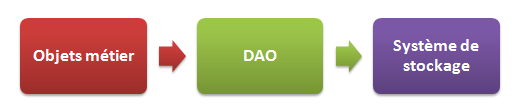
\includegraphics[scale=0.5]{../graph/dao1.png} \\
\end{center}

\subsubsection{Mise en place}
La couche DAO va gérer les opérations classiques de stockage : ajout, lecture, modification et suppression. Ces quatre opérations sont souvent raccourcis par l'acronyme CRUD (create, read, update and delete). \\

Pour mettre en application le modèle DAO nous avons du créer nos propres exceptions. En effet, il faut que les exceptions générées par SQL ou JDBC soit référencées comme étant des exceptions dues à la boite noire DAO. 

En reprenant la même idée, DAO se propose d'offrir une interface pour chacun des objets décrivant l'ensemble des méthodes qui seront accessibles dans l'objet. Ainsi, peu importe l'implémentation effectuée on pourra connaître les diverses méthodes de nos classes. Les interfaces permettent de décrire les méthodes des objets la couche donnée et ce n'est que l'implémentation qui sera dépendante du mode de stockage. Par exemple, pour un stockage SQL nous pouvons utiliser le driver JDBC présenté ci-dessus.\\ 
\begin{center}
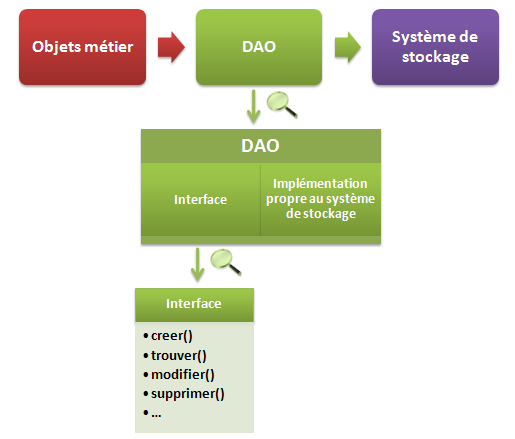
\includegraphics[scale=0.5]{../graph/dao2.png} \\
\end{center}

La couche DAO comportera également une fabrique. Cette fabrique sera unique et ne sera instanciée que si les informations de configuration sont correctes. Le but de cette fabrique sera de fournir une instance des différentes implémentations de la DAO.

\subsubsection{Avantage et Inconvénient}
L'avantage du modèle DAO est donc clair, le changement du stockage du mode de stockage de données est simple. En effet, nous aurons seulement à changer nos classes DAO pour changer ce mode de stockage. L'inconvénient est du à la mise en œuvre qui demande une couche supplémentaire. 


\subsection{La sérialisation}

\subsubsection{Principe}

La sérialisation est le processus de conversion d'un objet pour l'enregistrer dans une base de données ou un fichier par exemple. Le processus inverse s'appelle la désérialisation. Nous pouvons donc représenter cette méthode selon le schéma suivant. 

\begin{center}
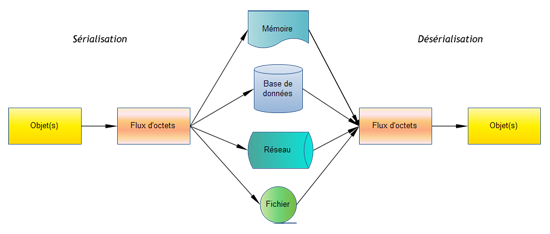
\includegraphics[scale=0.5]{../graph/serialisation.png} \\
\end{center}

\subsubsection{Mise en place}
On peut choisir par exemple d'effectuer sa sérialisation en XML. \\

La classe XMLEncoder permet de sérialiser un objet en XML. Cette sérialisation ne prend en compte que les champs ayant un getter et un setter public. XMLEncoder(output) crée une nouvelle instance qui utilise le flux passé en paramètre comme résultat de la sérialisation. \\

La classe XMLDecoder permet quand à elle de désérialiser un objet à partir d'un document XML. \\

Pour notre application nous aurions besoin d'effectuer une sérialisation vers SQL. Prenons l'exemple du joueur, pour effectuer la sérialisation nous avons besoin d'une classe Joueur qui implémente Serializable, d'avoir un constructeur par défaut et d'avoir un getter et un setter public pour chaque attribut. Ensuite notre table SQL java doit contenir un id et un longblob (Binary Large Object). Ensuite nous n'avons plus qu'a effectue une sauvegarde dans la base de données. Pour la desérialisation, il nous faut récupérer le longblob pour le convertir en ObjectInputStream pour utiliser la méthode readObject(). 


\subsubsection{Avantage et Inconvénient}
La sérialisation présente des avantages comme une bonne portabilité ou le fait que le processus de sérialisation ne prenne pas en compte les champs qui ont leur valeur par défaut. Elle présente les inconvénients suivants : 
\begin{itemize}
\item ne peut s'utiliser que sur des objets respectant la convention JavaBeans (constructeur par défaut, getter et setter pour tous les attributs ..)
\item la taille des données sérialisés est plus importante que leur équivalent binaire
\end{itemize}


\subsection{Notre choix : DAO vs Serialisation}
Pour la communication avec notre base de données nous avons choisi d'utiliser le modèle DAO. \\

Le modèle DAO demande plus de travail pour être mis en place que la sérialisation mais possède l'avantage de nous fournir une base de données plus facilement utilisable dans un autre contexte. En effet, chacune de nos tables ne seront pas simplement un blob mais une valeur pour chacun des champs de notre table. 